
%! program = pdflatex

\documentclass[12pt]{article}
\usepackage{amsmath}
\usepackage{natbib}
\usepackage{graphicx}
\usepackage{amssymb}
\usepackage{epstopdf}
\usepackage{float} % to keep the figures in place

\usepackage{color}
\newcommand{\cred}{ \color{red}}
\newcommand{\cgreen}{\color{green}}
\newcommand{\cblue}{\color{blue}}
\newcommand{\cmag}{\color{magenta}}
\newcommand{\bn}{\begin{enumerate}}
\newcommand{\en}{\end{enumerate}}
\newcommand{\bi}{\begin{itemize}}
\newcommand{\ei}{\end{itemize}}
\newcommand{\be}{\begin{eqnarray}}
\newcommand{\ee}{\end{eqnarray}}
\newcommand{\by}{\begin{eqnarray*}}
\newcommand{\ey}{\end{eqnarray*}}
\renewcommand{\labelenumi}{(\alph{enumi}) }
%
\usepackage[margin=2.2cm, includehead]{geometry}% see geometry.pdf on how to lay out the page. There's lots.
\geometry{letterpaper} % or letter or a5paper or ... etc
% \geometry{landscape} % rotated page geometry
%\bibpunct{(}{)}{;}{a}{,}{,}
%\setlength{\textwidth}{16cm}
%\setlength{\textheight}{21cm}
\def\nonumber{\global\@eqnswfalse}
\newcounter{parnum}
\newcommand{\N}{%
  \noindent\refstepcounter{parnum}%
   \makebox[\parindent][l]{\textbf{[\arabic{parnum}]}}\quad  }
% Use a generous paragraph indent so numbers can be fit inside the
% indentation space.
\setlength{\parindent}{1.5em}

% See the ``Article customise'' template for come common customisations

\date{}
%\date{} % delete this line to display the current date

%%% BEGIN DOCUMENT
\usepackage{Sweave}
\begin{document}
\Sconcordance{concordance:HW7.tex:HW7.Rnw:%
1 47 1 1 0 24 1 1 2 1 0 2 1 4 0 1 2 12 1 1 2 1 0 1 1 25 0 1 2 5 1 1 4 1 %
2 4 1 1 2 5 0 1 2 1 1 1 2 5 0 1 2 12 1 1 2 1 0 2 1 38 0 1 2 2 1 1 4 1 2 %
12 1 1 2 1 0 1 1 32 0 1 2 2 1 1 2 1 0 2 1 4 0 1 2 7 1 1 3 1 2 4 1 1 2 8 %
0 1 2 2 1 1 2 1 0 9 1 7 0 1 2 3 1 1 2 1 0 3 1 7 0 1 2 4 1 1 2 1 0 3 1 8 %
0 2 2 7 0 2 2 1 0 4 1 5 0 6 1 8 0 1 1 9 0 1 2 4 1}

%\large
%\maketitle
\newtheorem{thm}{Theorem}[section]
\newtheorem{cor}[thm]{Corollary}
\newtheorem{lem}[thm]{Lemma}
\newtheorem{prop}[thm]{Proposition}
\newtheorem{defn}[thm]{Definition}
\newtheorem{exam}[thm]{Example}
\newtheorem{qstn}[thm]{Question}

%%%
\newpage
\begin{center}
{\bf Homework 7 - STAT 511}\\
Amal Agarwal
\end{center}
%==========================
\section*{Answer 1}
\bn
\item
\begin{itemize}
\item The given data was extracted and exploratory data analysis was conducted by plotting pairwise scatter plots. In particular the plot of consumption vs. date indicates positive autocorrelation as can be seen by the following plot:
\begin{figure}[H]
\begin{Schunk}
\begin{Sinput}
> ice=read.csv("icecream.csv",sep=",")
> plot.ts(ice$IC)
> ice<-ice[-length(ice$date),]
\end{Sinput}
\end{Schunk}
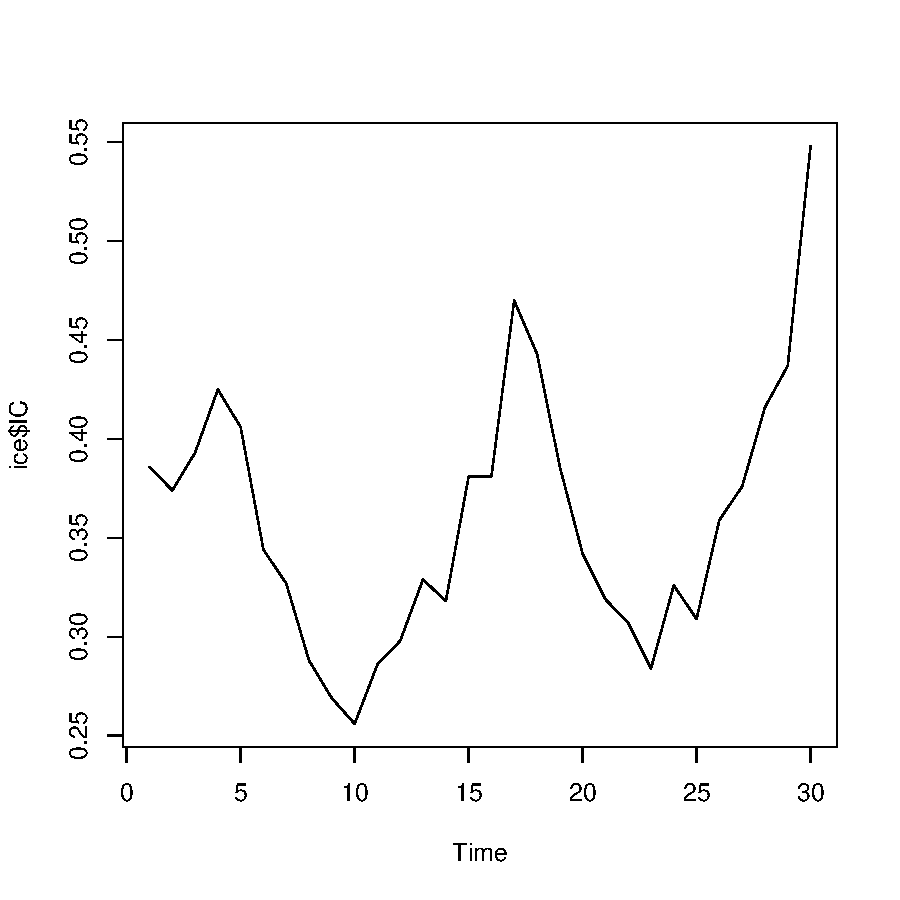
\includegraphics{HW7-001}
\end{figure}

Fitting a simple linear model 

\begin{equation*}
\begin{aligned}
IC_{i} &= \beta_0 + \beta_1 date_{i} +  \beta_2 price_{i} + \beta_3 income_{i} + \beta_4 temp_{i} + \epsilon_{i}
\end{aligned}
\end{equation*}
where $\epsilon_{i} \sim N(0,\sigma^2)$\\

and observing the summary as 

\begin{Schunk}
\begin{Sinput}
> fit1=lm(IC~.,data=ice)
> summary(fit1)
\end{Sinput}
\begin{Soutput}
Call:
lm(formula = IC ~ ., data = ice)

Residuals:
      Min        1Q    Median        3Q       Max 
-0.059458 -0.015630  0.005229  0.017152  0.070472 

Coefficients:
              Estimate Std. Error t value Pr(>|t|)    
(Intercept)  8.666e-02  3.082e-01   0.281    0.781    
date        -8.898e-06  1.478e-03  -0.006    0.995    
price       -3.854e-01  8.141e-01  -0.473    0.640    
income       2.629e-03  2.133e-03   1.233    0.230    
temp         3.120e-03  4.419e-04   7.060 2.68e-07 ***
---
Signif. codes:  0 ‘***’ 0.001 ‘**’ 0.01 ‘*’ 0.05 ‘.’ 0.1 ‘ ’ 1 

Residual standard error: 0.03359 on 24 degrees of freedom
Multiple R-squared: 0.6948,	Adjusted R-squared: 0.6439 
F-statistic: 13.66 on 4 and 24 DF,  p-value: 6.102e-06 
\end{Soutput}
\end{Schunk}

we can infer the following things:
\begin{itemize}
\clearpage
\item Plotting the reiduals vs. date we get,
\begin{figure}[H]
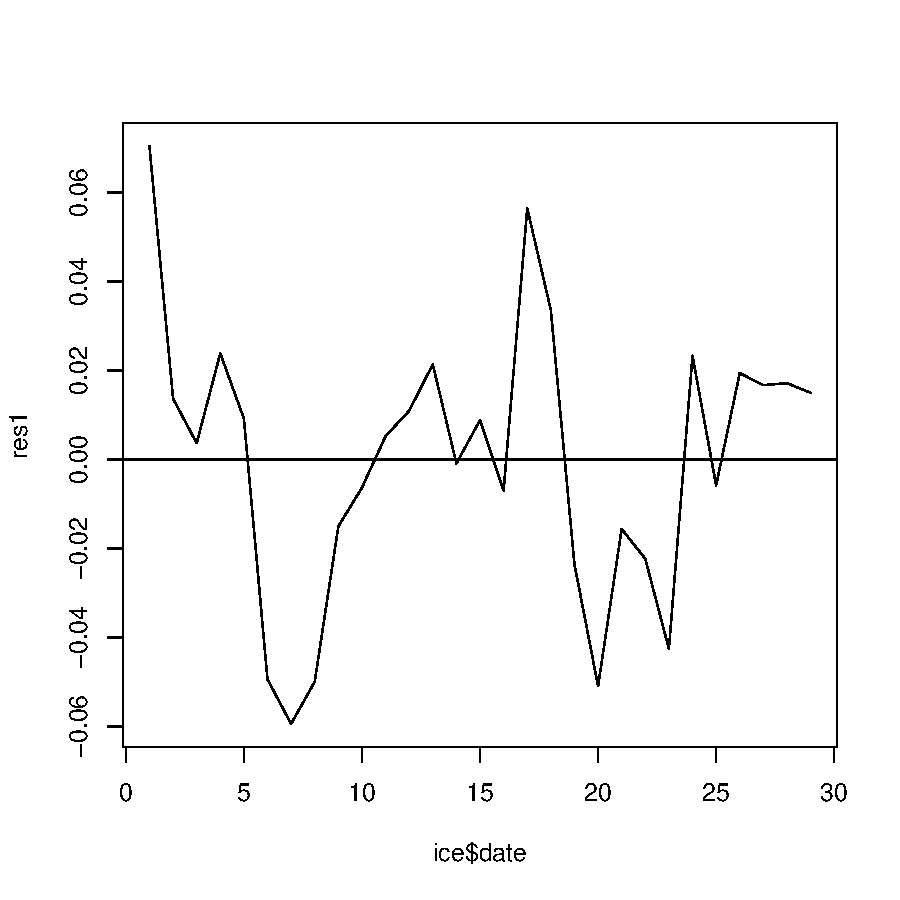
\includegraphics{HW7-003}
\end{figure}
The above residual plot clearly confirms our hypothesis of positive autocorrelation under the fitted model. However, it also indicates a global periodic trend and suggests that if we include a sine/cosine term, we might be able to use our normal uncorrelated errors model.\\
\clearpage
\item Testing for the autocorrelation:
\begin{figure}[H]
\begin{Schunk}
\begin{Sinput}
> acf(res1)
\end{Sinput}
\end{Schunk}
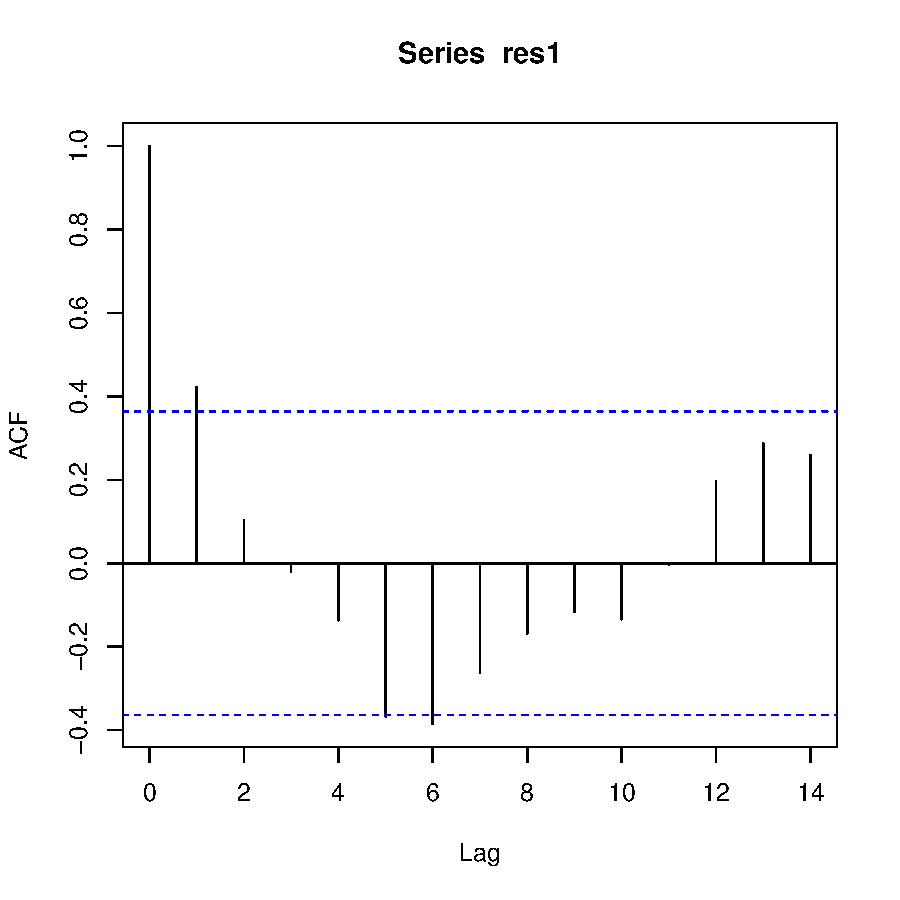
\includegraphics{HW7-004}
\end{figure}
\begin{figure}[H]
\begin{Schunk}
\begin{Sinput}
> pacf(res1)
\end{Sinput}
\end{Schunk}
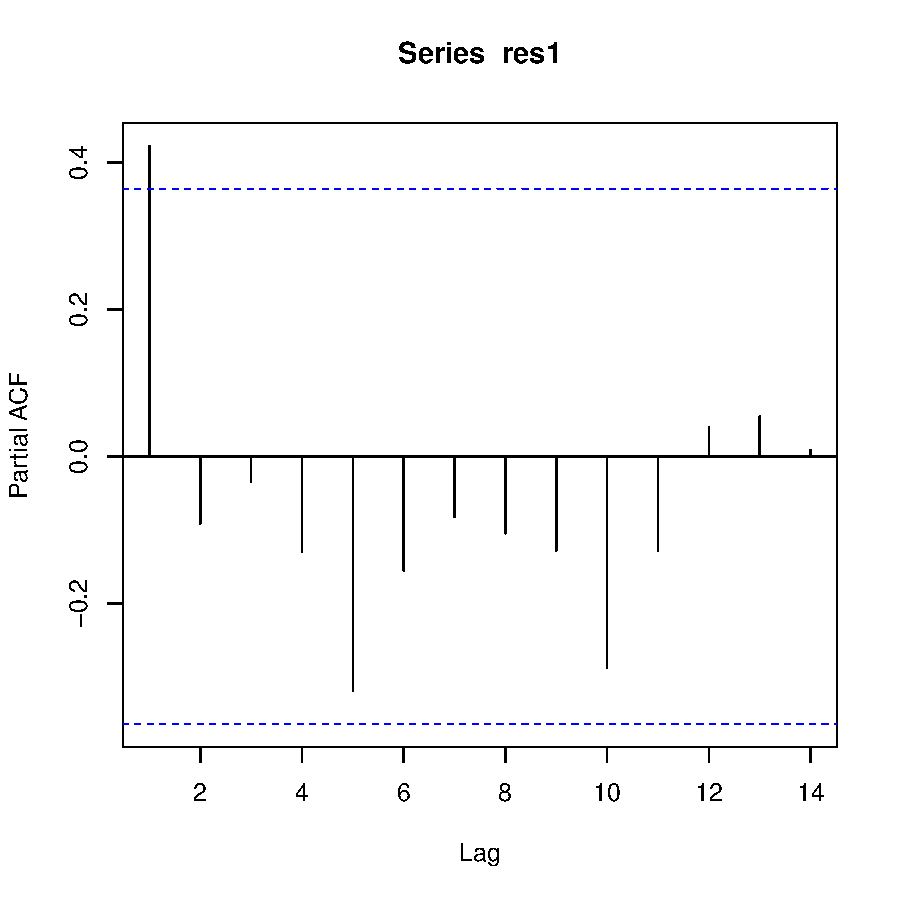
\includegraphics{HW7-005}
\end{figure}
\end{itemize}
Tis confirms that only lag-1 autocorrelation is significant and so we can use an AR(1) time series model.

\item Now fitting the following AR(1) correlated errors linear model: 

\begin{equation*}
\begin{aligned}
IC &= \beta_0 + \beta_1 date +  \beta_2 price + \beta_3 income + \beta_4 temp + \epsilon
\end{aligned}
\end{equation*}
where $\epsilon \sim N(0,\Sigma), \Sigma_{ij}=\dfrac{\sigma_u^2}{1-\rho^2}\rho^{|i-j|}$\\

\begin{Schunk}
\begin{Sinput}
> library(nlme)
> fit2=gls(IC~.,data=ice,correlation=corAR1(),method="REML")
> summary(fit2)
\end{Sinput}
\begin{Soutput}
Generalized least squares fit by REML
  Model: IC ~ . 
  Data: ice 
        AIC       BIC   logLik
  -76.34285 -68.09647 45.17142

Correlation Structure: AR(1)
 Formula: ~1 
 Parameter estimate(s):
      Phi 
0.8757438 

Coefficients:
                 Value Std.Error   t-value p-value
(Intercept)  0.5358471 0.2630945  2.036709  0.0529
date         0.0010757 0.0030762  0.349682  0.7296
price       -0.6250332 0.6652191 -0.939590  0.3568
income      -0.0015569 0.0019697 -0.790421  0.4370
temp         0.0024662 0.0006535  3.773659  0.0009

 Correlation: 
       (Intr) date   price  income
date    0.089                     
price  -0.774 -0.040              
income -0.687 -0.345  0.136       
temp   -0.224 -0.150  0.028  0.170

Standardized residuals:
       Min         Q1        Med         Q3        Max 
-1.3961197 -0.6097035 -0.2332330  0.2828391  0.6459124 

Residual standard error: 0.05908097 
Degrees of freedom: 29 total; 24 residual
\end{Soutput}
\end{Schunk}
\clearpage
Checking the residual plot again:
\begin{figure}[H]
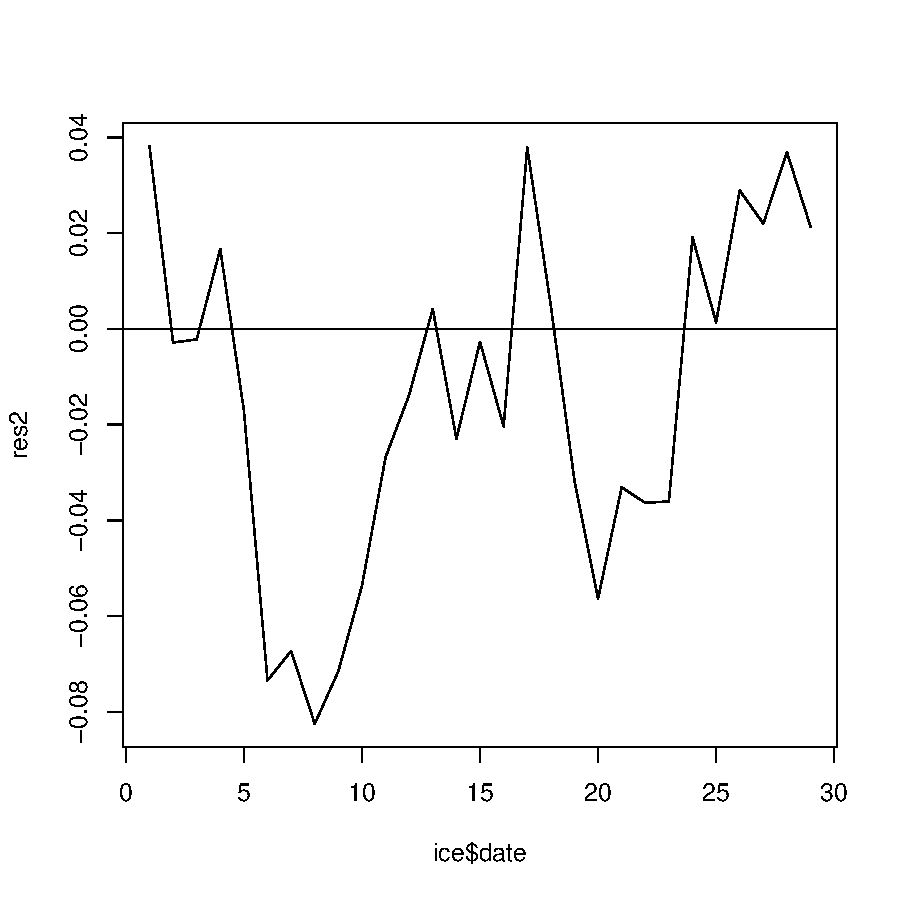
\includegraphics{HW7-007}
\end{figure}
The above plot looks much more better.
Based on the summary of the fit, it is clear that the p-values for the date, price and income are very large (greater than 0.05 significance criteria) which suggests that these predictor variables are not statistically significant in explaining the variation in consumption. Thus, these variables can be dropped from the model.\\

\item Fitting the following correlated errors linear model:

\begin{equation*}
\begin{aligned}
IC &= \beta_1 temp + \epsilon
\end{aligned}
\end{equation*}
where $\epsilon \sim N(0,\Sigma), \Sigma_{ij}=\dfrac{\sigma_u^2}{1-\rho^2}\rho^{|i-j|}$\\

\begin{Schunk}
\begin{Sinput}
> fit3=gls(IC~temp,data=ice,correlation=corAR1(),method="REML")
> summary(fit3)
\end{Sinput}
\begin{Soutput}
Generalized least squares fit by REML
  Model: IC ~ temp 
  Data: ice 
        AIC       BIC  logLik
  -101.0608 -95.87745 54.5304

Correlation Structure: AR(1)
 Formula: ~1 
 Parameter estimate(s):
      Phi 
0.7557313 

Coefficients:
                 Value  Std.Error  t-value p-value
(Intercept) 0.23545840 0.03462528 6.800188   0e+00
temp        0.00260358 0.00059407 4.382617   2e-04

 Correlation: 
     (Intr)
temp -0.842

Standardized residuals:
       Min         Q1        Med         Q3        Max 
-1.6894484 -0.7887911 -0.1756249  0.4859311  1.1391942 

Residual standard error: 0.04133097 
Degrees of freedom: 29 total; 27 residual
\end{Soutput}
\end{Schunk}
\clearpage
Checking the residual plot again:
\begin{figure}[H]
\begin{Schunk}
\begin{Sinput}
> res3=resid(fit3)
> plot(res3,type='l')
> abline(h=0)
\end{Sinput}
\end{Schunk}
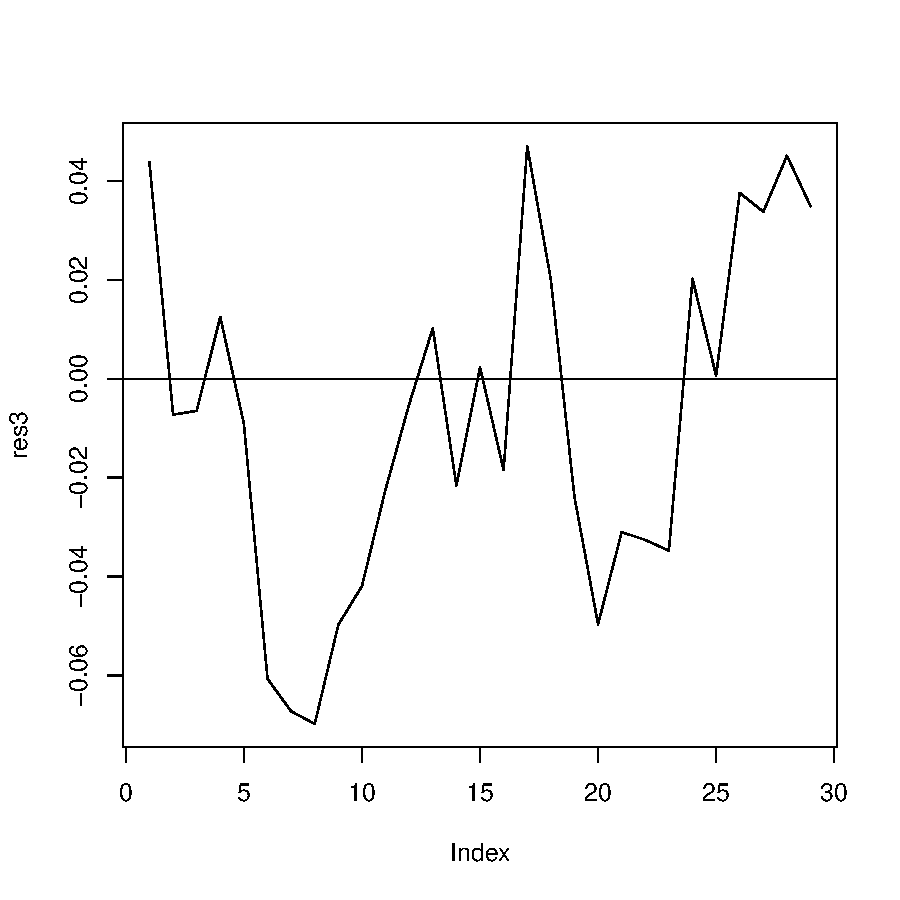
\includegraphics{HW7-009}
\end{figure}
The residual plot looks good now since the positive autocorrelation has been taken into account. There is no visible non-linear trend.\\

Clearly the estimate of $\rho$ in our model is 0.7557313 which indicates a high postive lag 1 autocorrelation.

\clearpage
The qq plot of residuals is given as:
\begin{figure}[H]
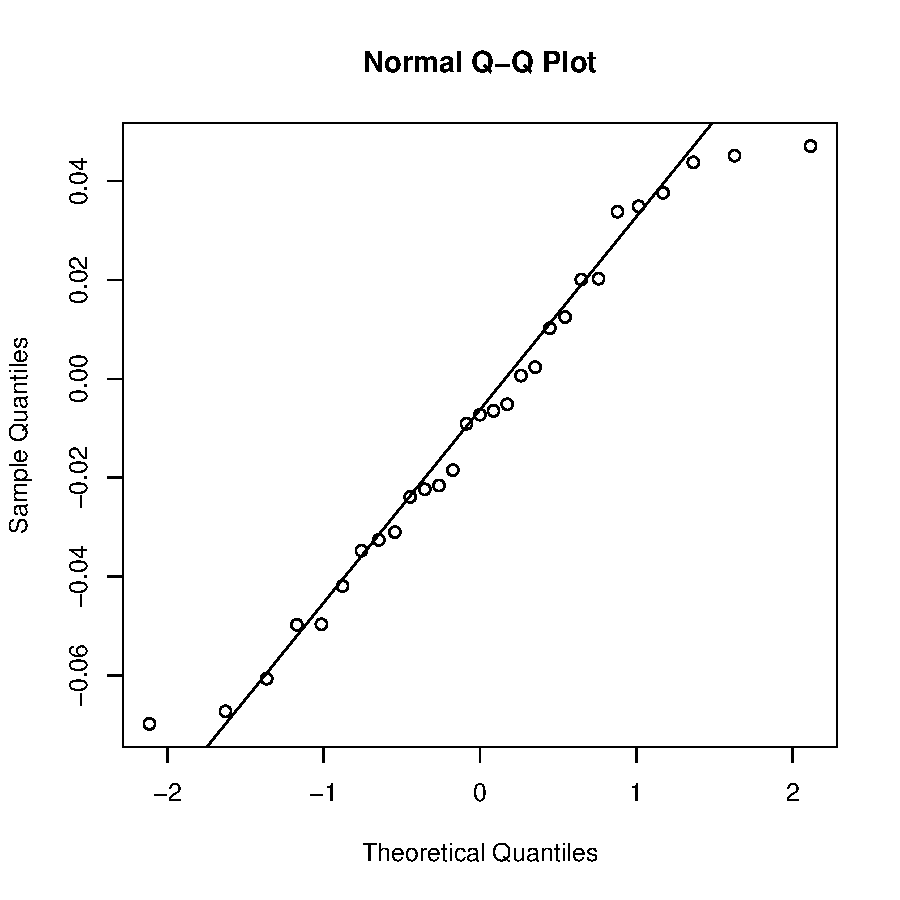
\includegraphics{HW7-010}
\end{figure}

The above plot shows some short tails which are not significant. Hence our normality assumption is satisfied.

The estimated coeffiecients are given as:
\begin{Schunk}
\begin{Sinput}
> fit3$coeff
\end{Sinput}
\begin{Soutput}
(Intercept)        temp 
0.235458396 0.002603578 
\end{Soutput}
\end{Schunk}

The positive slope of 0.002 shows that the mean consumption increases by 0.002 units with a unit increase in temperature. The postive value of intercept indiactes that the consumption at zero temperature. Note that the temperature is in Fahrenheit and thus it makes sense that even at $0^0$ F, the consumtion is 0.235 units. Further the estimated value of the nuisance parameter $\sigma_u^2$ is 

\begin{Schunk}
\begin{Sinput}
> X=cbind(1,ice$temp)
> n=29
> p=2
> rho.hat=0.7557313
> C.ar1=corAR1(rho.hat)
> C.ar1=Initialize(C.ar1,data=ice)
> R=corMatrix(C.ar1)
> W=solve(R[1:29,1:29]/(1-(rho.hat)^2))
> sigma2<-(t(res3)%*%W%*%res3)/(n-p)
> sigma2
\end{Sinput}
\begin{Soutput}
             [,1]
[1,] 0.0007326174
\end{Soutput}
\end{Schunk}

\end{itemize}
\clearpage
\item Using the procedure mentioned above, the p-value under t distribution for $H_0: \beta_1=0$ can be calculated as
\begin{Schunk}
\begin{Sinput}
> Y<-solve(t(X)%*%W%*%X)
> F<-(as.numeric(fit3$coeff[2])^2)/(Y[2,2]*sigma2)
> p_val<-2*(1-pt((sqrt(F)),(n-p)))
> p_val
\end{Sinput}
\begin{Soutput}
             [,1]
[1,] 0.0001598054
\end{Soutput}
\end{Schunk}

Note that this caluclated p value  is same as the p value obtained from the summary of fitting the final model i.e. summary of fit 3 shown earlier.

\clearpage
\item The predicted value at date=30 calculated using predict function is given as:
\begin{Schunk}
\begin{Sinput}
> ice=read.csv("icecream.csv",sep=",")
> newdata=ice[30,]
> Y30_cap=predict(fit3, newdata)
> Y30_cap
\end{Sinput}
\begin{Soutput}
[1] 0.4203124
attr(,"label")
[1] "Predicted values"
\end{Soutput}
\end{Schunk}
which is slightly different from the true response 
\begin{Schunk}
\begin{Sinput}
> ice$IC[30]
\end{Sinput}
\begin{Soutput}
[1] 0.548
\end{Soutput}
\end{Schunk}
The prediction interval an be calculated as:
\begin{Schunk}
\begin{Sinput}
> H=X%*%Y%*%t(X)%*%W
> I=diag(1,29)
> V=((I-H)%*%solve(W)%*%t(I-H))
> h29<-V[29,29]
> h29
\end{Sinput}
\begin{Soutput}
[1] 1.748117
\end{Soutput}
\begin{Sinput}
> X30=matrix(c(1,ice$temp[30]),nrow=1,ncol=2)
> cf=(1/(1-rho.hat^2))+((rho.hat^2)*h29)+(X30%*%Y%*%t(X30))
> s=sqrt(fit3$sigma^2*cf)
> U=Y30_cap+s*qt(0.975,(n-p))
> L=Y30_cap-s*qt(0.975,(n-p))
> L
\end{Sinput}
\begin{Soutput}
          [,1]
[1,] 0.2499013
attr(,"label")
[1] "Predicted values"
\end{Soutput}
\begin{Sinput}
> U
\end{Sinput}
\begin{Soutput}
          [,1]
[1,] 0.5907236
attr(,"label")
[1] "Predicted values"
\end{Soutput}
\end{Schunk}

Clearly the lower bound L=0.2499013 and upper bound U=0.5907236 contains the true response=0.548 at date=30.

\en
\end{document}
